\textbf{6-1.}在给定的坐标系下, 设力 $F = 3i + 4k$ 的作用点位置矢量为: $\mathbf{r} = 2\mathbf{j} - 6\mathbf{k}$ , 其中 $\mathbf{F}$ 以 $\mathbf{N}$ 为单位, $\mathbf{r}$ 以 $\mathrm{m}$ 为单位, 求力对坐标原点的力矩。

\vfill

\textbf{6-2.}若将地球绕太阳的公转看作是以太阳为中心的圆周运动,试求地球相对太阳中心的角动量。已知地球的质量 $m_{\mathrm{E}} = 6.0 \times 10^{24} \mathrm{~kg}$ , 轨道半径 $R = 1.49 \times 10^{11} \mathrm{~m}$ 。

\vfill
\newpage

\textbf{6-3.}一质量 $m = 2 \mathrm{~kg}$ 的质点由静止开始做半径 $R = 5 \mathrm{~m}$ 的圆周运动。其相

对圆心的角动量随时间的变化关系为 $L=3t^{2}$ ，角动量 L 的单位为 $kg \cdot m^{2}/s, t$ 的单位为 s。

试求:(1) 质点受到的相对于圆心的力矩;

(2) 质点运动角速度随时间的变化关系。

\vfill

\textbf{6-4.}如习题 6-4 图所示, 一根轻绳跨过具有光滑水平轴的定滑轮(质量可忽略), 两个质量分别为 $m_{1}$ 和$m_{2}$ 的人各抓住绳子的一端。开始时，两人与水平轴之间的高度差分别为 $h_{1}$ 和 $h_{2}$ ，他们同时开始向上爬，并同时到达该滑轮的水平轴处。试求他们爬绳所经历的时间 t。

\begin{figure}[H]
  \centering
  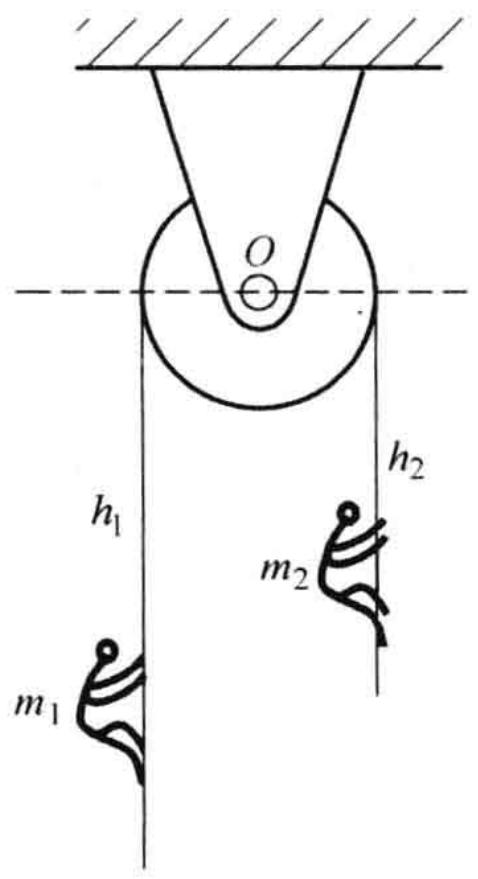
\includegraphics[width=0.2\textwidth]{figures/fig6-4.jpg}
  \end{figure}

\vfill
\newpage

\textbf{6-5.}在光滑的水平面上, 用长为 $l$ 的轻线连接两个质量分别为 $m_{1}$ 和 $m_{2}$ 的小球。开始时, 线正好拉直, $m_{1}$ 和 $m_{2}$ 的速度分别为 $v_{1}$ 和 $v_{2} (v_{1} > v_{2})$ , 它们的方向相同, 且垂直于连线。试问:

(1) 系统相对质心的角动量为多大?

(2) 线中的张力为多大?

\begin{figure}[H]
  \centering
  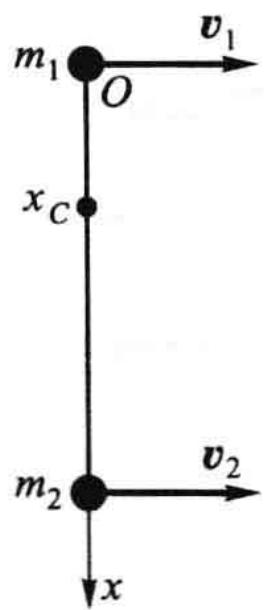
\includegraphics[width=0.1\textwidth]{figures/fig6-5.jpg}
  \end{figure}

\vfill

\textbf{6-6.}两个质量均为 $60 \mathrm{~kg}$ 的滑冰者, 在两条相距 $10 \mathrm{~m}$ 的平直跑道上以 $6.5 \mathrm{~m} / \mathrm{s}$ 的速率沿相反方向匀速滑行。当他们之间的距离恰好等于 $10 \mathrm{~m}$ 时, 他们分别抓住一根长 $10 \mathrm{~m}$ 的绳子的两端。若将滑冰者看成质点, 并略去绳子的质量。

(1) 求他们抓住绳子前后相对于绳子中点的角动量;

(2) 两人都用力缓慢往自己这边拉绳子, 当他们之间的距离为 $5 \mathrm{~m}$ 时, 各自的速率是多大?

(3) 求此时绳中的张力；

(4) 计算每个人在拉绳过程中所做的功。

\vfill
\newpage

\textbf{6-7.}一颗人造地球卫星沿椭圆轨道绕地球运行。在近地点, 卫星与地球中心的距离为地球半径的 3 倍。而在近地点, 卫星的速度为在远地点时的 4 倍。求在远地点时卫星与地球中心之间的距离为地球半径的多少倍。

\vfill

\textbf{6-8.}由火箭将一颗人造卫星送入离地面很近的轨道, 进入轨道时, 卫星的速度方向平行于地面, 其大小为在地面附近做圆周运动的速度的 $\sqrt{1.5}$ 倍。试求该卫星在运行中与地球中心的最远距离。

\vfill
\newpage

\textbf{6-9.}试求月球表面的重力加速度和从月球表面逃逸的速度。已知月球的半径 $R_{\text{月球}} = 1.7 \times 10^{6} \mathrm{~m}$ , 月球的质量 $m_{\text{月球}} = 7.3 \times 10^{22} \mathrm{~kg}$ 。

\vfill

\textbf{6-10.}在光滑水平桌面上, 质量分别为 $m_0$ 和 $m$ 的两物体系于原长为 $a$ , 劲度系数为 $k$ 的弹簧的两端。现使 $m_0$ 获得一与弹簧垂直的速度 $v_0$ 。试证明: 若 $v_0 = 3a \sqrt{\frac{k}{2m'}}$ , 其中 $m'$ 为约化质量, 则在以后的运动过程中两物体之间的最大距离为 $3a$ 。

\vfill
\newpage


\textbf{6-11.}发射一宇宙飞船去考察一质量为 $m_{0}$ 、半径为 $R$ 的行星。当飞船静止于空间离行星中心 $5 R$ 处时, 以速度 $v_{0}$ 发射一包仪器, 如习题 6-11 图所示。仪器包的质量 $m$ 远小于飞船的质量, 要使该仪器包恰好掠擦行星表面着陆, $\theta$ 角应是多少?

\begin{figure}[H]
  \centering
  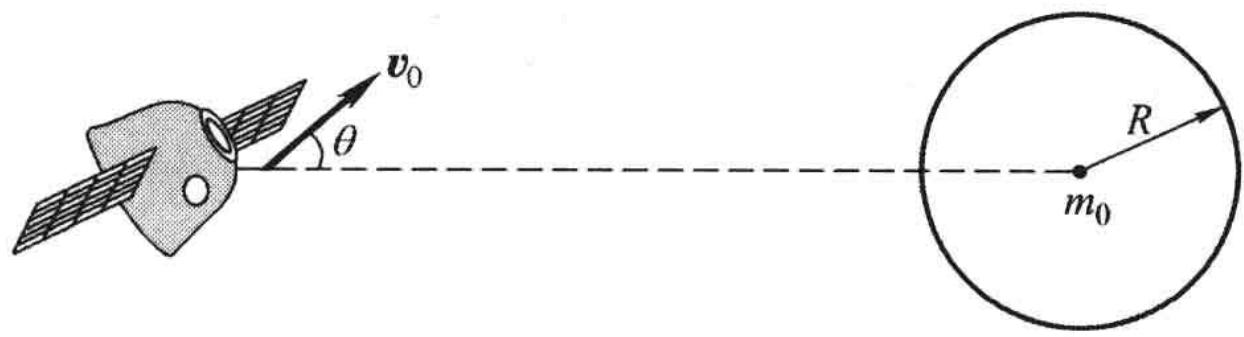
\includegraphics[width=0.4\textwidth]{figures/fig6-11_6.jpg}
  \end{figure}

\vfill

\textbf{6-12.}一质量为 $m$ 的空间站沿半径为 $r$ 的圆周绕月球运动。为使空间站能

在月球上登陆,当空间站运行至轨道上 P 点时向前发射一质量为 $m_{1}$ 的物体,来改变空间站的运行速度,从而使其沿习题 6-12 图所示的新轨道运动,并在月球表面登陆。已知月球的半径为 $R_{月}$ ,月球的质量为 $m_{月}$ ,试求 $m_{1}$ 的发射速度 $v_{1}$ (相对月球参考系)。

\begin{figure}[H]
  \centering
  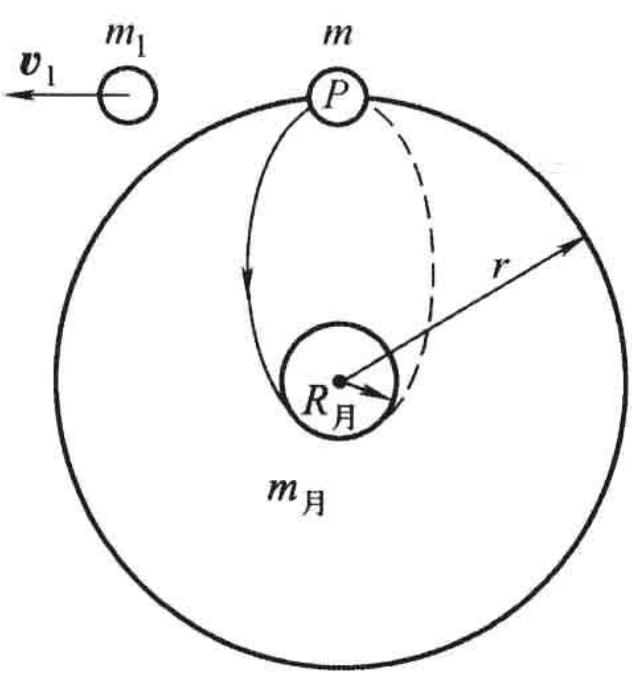
\includegraphics[width=0.23\textwidth]{figures/fig6-12.jpg}
  \end{figure}

\vfill
\newpage

\textbf{6-13.}质量为 $m$ 的质点在质量为 $m_0$ 的质点（视为固定）的引力场中以 $m_0$ 为中心做半径为 $r_0$ 的周期运动。若给 $m$ 以沿径向的冲量 $I$ , 并设 $I$ 与质点的原动量之比为一小量, 求 $m$ 在以后运动过程中径矢的最大值 $r_2$ 与最小值 $r_1$ , 并证明在忽略二级以上小量的情况下, $r_2 - r_0 \approx r_0 - r_1$ , 即质点 $m$ 的运动轨道近似为一偏心的圆。

\vfill

\textbf{6-14.}天狼星是天空中最明亮的恒星,因此人们很早就已开始观察它的运动。1844年德国天文学家弗里德里希·贝塞尔注意到天狼星运动的异常情况,并据此预言它附近有伴星。1862年美国阿尔文·克拉克首次观测到这一伴星(系白矮星,肉眼看不到)。根据以后的观测资料,该双星系统的运动轨迹如习题6-14图所示。图中粗、细实线分别表示天狼星与其伴星的运动轨迹,虚线为质心的运动轨迹,第一组黑点表示1862年的双星位置,其余各组黑点分别表示自1870年起至1940年每隔10年的双星位置。天狼星和伴星的平均距离为

s=20.4 AU(1 AU=1.496×10 $^{8}$ km)，它们与质心的距离之比约为2:5。

(1) 由图判断双星在相对做圆周运动还是椭圆运动? 运动周期是多少年?

(2) 假定双星相对做距离为 $a$ 的匀速圆周运动, 试估算天狼星及其伴星的质量 $m_{\mathrm{A}}$ 和 $m_{\mathrm{B}}$ (用太阳质量 $m_{\mathrm{S}}$ 表示)。

\begin{figure}[H]
  \centering
  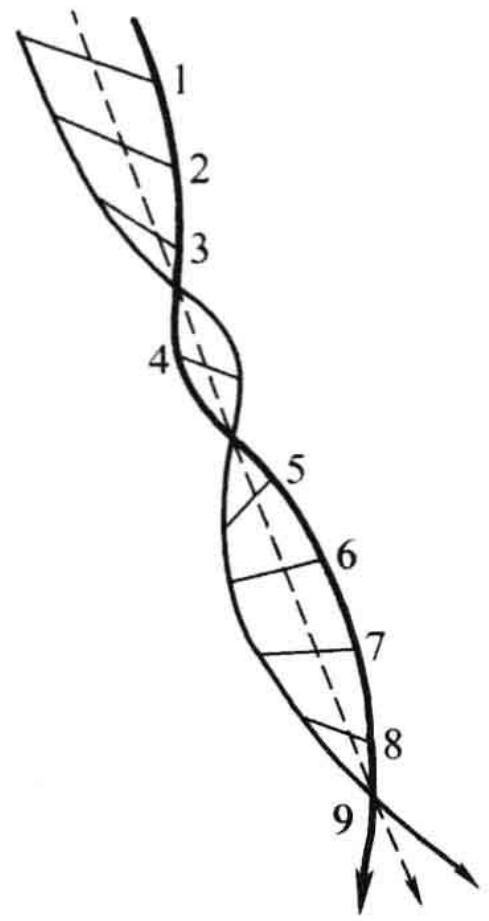
\includegraphics[width=0.18\textwidth]{figures/fig6-14.jpg}
  \end{figure}

\vfill
\newpage

\textbf{6-15.}如习题 6-15 图所示, 质量均为 $m$ 的小球 1、2 用长为 $4a$ 的细线相连, 以速度 $v$ 沿着与线垂直的方向在光滑水平台面上运动, 线处于伸直状态。在运动过程中, 线上距离小球 1 为 $a$ 的一点与固定在台面上的一竖直光滑细钉相碰, 设在以后的运动过程中两球不相碰。求:

(1) 小球 1 与钉的最大距离；

(2) 线中的最小张力。

\begin{figure}[H]
  \centering
  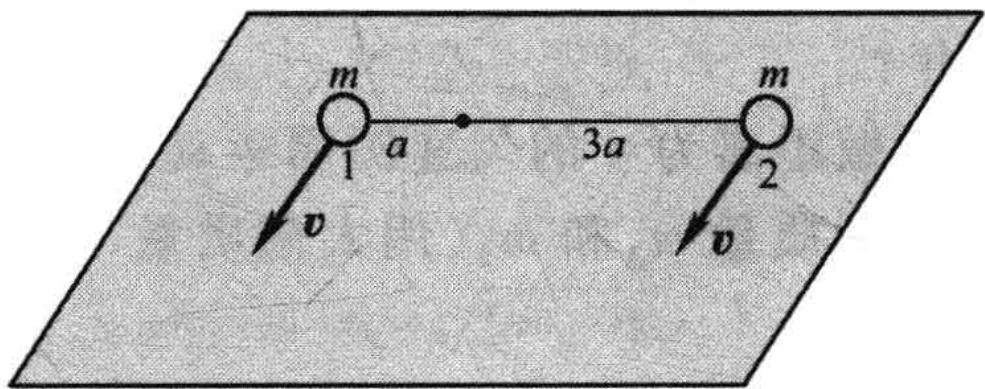
\includegraphics[width=0.28\textwidth]{figures/fig6-15.jpg}
  \end{figure}

\vfill

\textbf{6-16.}在一半径为 $R = 2.0 \times 10^{8} \mathrm{~m}$ 的无空气的星球表面, 若以 $v_{0} = 10 \mathrm{~m} / \mathrm{s}$ 的速度竖直上抛一物体, 则该物体上升的最大高度为 $h = 8 \mathrm{~m}$ 。试问:

(1) 该星球的逃逸速度有多大?

(2) 若要使该星球成为黑洞,则现有的半径应比黑洞的半径大几倍?

(本题可参考第十二章 12.3.5 节有关黑洞的介绍)

\vfill
\newpage